\documentclass[]{mwart}

\usepackage{polski}
\usepackage[utf8]{inputenc}

\usepackage{amsthm}
\usepackage{amsmath}
\usepackage{amssymb}

\usepackage{mdframed}
\usepackage{hyperref}
\usepackage[draft%      % dla obrazkow zakomentowac draft
]{graphicx}  
\usepackage{url}
\usepackage{enumitem}


\usepackage{caption}    
\usepackage{float}      



\usepackage{fancyhdr}
\pagestyle{fancy}
\fancyhf{}

\fancyhead[L]{
\includegraphics[height=0.666cm]{logo_projektu.png}}
\fancyhead[C]{\textit{Poprawa jakości zdjęć}}
\fancyhead[R]{
\includegraphics[height=0.9cm]{logo_uczelni.png}}
\fancyfoot[C]{\thepage}

\setlength{\headheight}{20pt}  



\usepackage{listings}
\usepackage{xcolor} 




\begin{document}
\thispagestyle{empty}

\begin{figure}[h]
    \centering
    
\includegraphics[width=1\textwidth]{logo_uczelni.png}
\end{figure}


\begin{center}
    {\LARGE \textbf{Poprawa jakości skanów zdjęć wykonanych techniką analogową
        }} \\[0.3cm]
    {\large \textbf{Raport II}} \\[0.2cm]
    \textit{projekt realizowany pod opieką prof. dr hab. inż. Artura Przelaskowskiego}

\end{center}

\begin{figure}[h]
    \centering
    
\includegraphics[width=1\textwidth]{logo_projektu.png}
\end{figure}

\vfill
\begin{abstract}
    Raport 2 projektu poprawy jakości zdjęć wykonanych analogowych przez grupę wtorkową z godziny 18
    w składzie:  Bartosz Wójcik, Katarzyna Szwed, Natalia Szymańska,
    Patrycja Szałajko, Aleksandra Wójcik, Karol Sęk, Michał Juszkiewicz, Filip Sajko.

    W tym raporcie zredefiniujemy cel naszego projektu i opiszemy problem z którym się mierzymy.
    Przedstawimy ponadto wstępną wersję naszego programu i zademonstrujemy jego skuteczność.
\end{abstract}

\newpage
\tableofcontents{}

\newpage

\section{Cel projektu}
W związku ze słusznymi uwagami i wskazówkami, podjelismy decyzję o ukonkretyzowaniu celu naszego projektu.
Skupimy się przede wszystkim na poprawianiu defektów cyfrowych skanów zdjęć analogowych.
Staramy się trafić do dwóch (niekoniecznie rozłącznych) grup osób --
współczesnych fanów fotografii analogowej (będącą dla amatora niełatwą sztuką) i posiadaczy pękatych
archiwów zdjęć rodzinnych chcących je zachować i cyfrowo utrwalić.

\section{Zdjęcia, zdjęcia!}
Profilowym zdjęciem dla nas jest portret -- tak inwidualny jak i grupowy.
Jest to typ zdjęć najbardziej popularny w rodzinnych albumach -- mnogość w nich zdjęć z ważnych
dla danej familli wydarzeń: chrztów, wesel czy pogrzebów... Służą one utrwaleniu wspomnień oraz pamięci
po krewnych i bliskich którzy już odeszli... A więc noszących dużą wartość emocjonalną dla ich posiadacza.

Przykładem takiej osoby jest nasza koleżanka Ola -- wraz z jej rodzinnym albumem.

\section{Problemy}
Wykonywanie, a następnie `ucyfrowienie' zdjęcia w technice analogowej wiąże się z różnymi trudnościami,
które mogą znacząco obniżyć jakość zdjęcia -- a z tym satysfakcje jego posiadacza. Głównymi problemami
którym będziemy przeciwdziałać będą niedoświetlenie zdjęcia i zanieczyszczenia powietrza osadzające
się na oryginalnym zdjęciu i skanerze podczas procesu `ucyfrowienia' go.

\subsection{Niedoświetlenie} % tak wiem bartek bedziesz krzyczal. ale poezja to poezja, e viva latre
Niedoświetlenie jest problemem trudnym -- zwłaszcza dla fanów-amatorów techniki analogowej.
Zasadnicza większość klasycznych aparatów nie posiada zaawansowanej mechaniki automatycznie wybierającej
odpowiednie ustawienia aparatu, a brak możliwości podglądu tego, jak dane zdjęcie wyszło często doprowadza
do sytuacji, gdzie po wielu dniach okazuje się, że na zdjęciu chwili którą fotograf chciał uchwycić i utrwalić
niewiele widać, bo przez złe ustawienia większość szczegółów jest niewidoczna...\footnote{Jest to problem który szeroko
    wraz z przykładami i analizą numeryczną opisywaliśmy w raporcie pierwszym.}
Dla przykładu przypomnijmy:
\newpage
\begin{figure}[H]
    \centering
    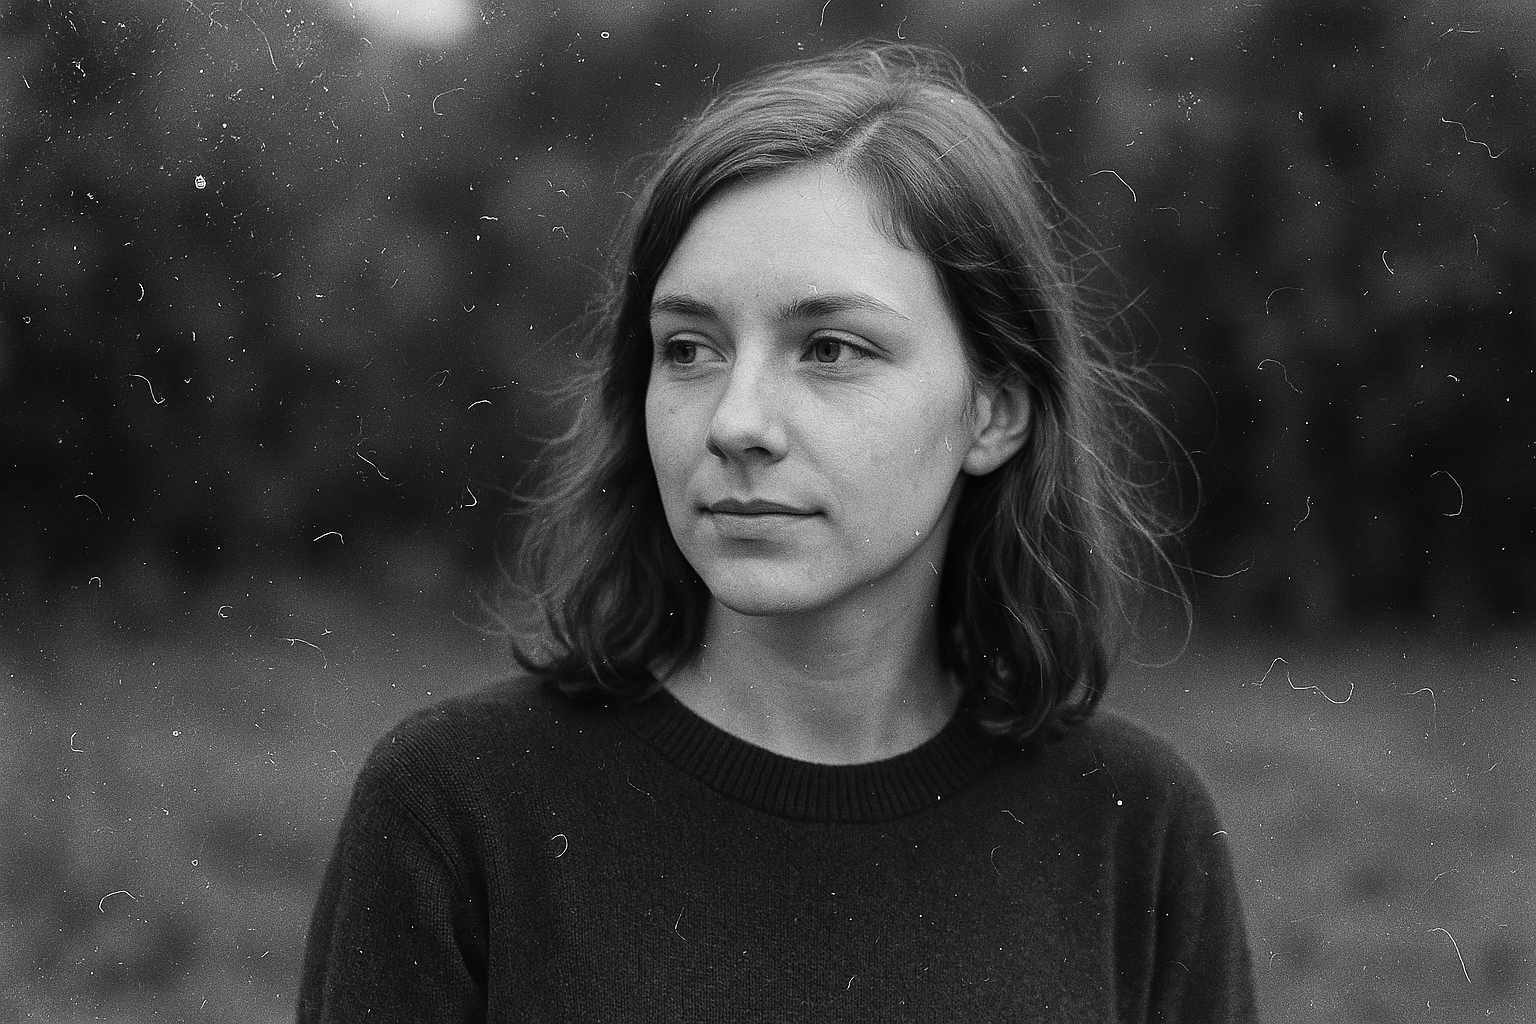
\includegraphics[width=\linewidth, keepaspectratio]{p_1.jpg}
    \caption{Zdjęcie niedoświetlone}
\end{figure}
\begin{figure}[H]
    \centering
    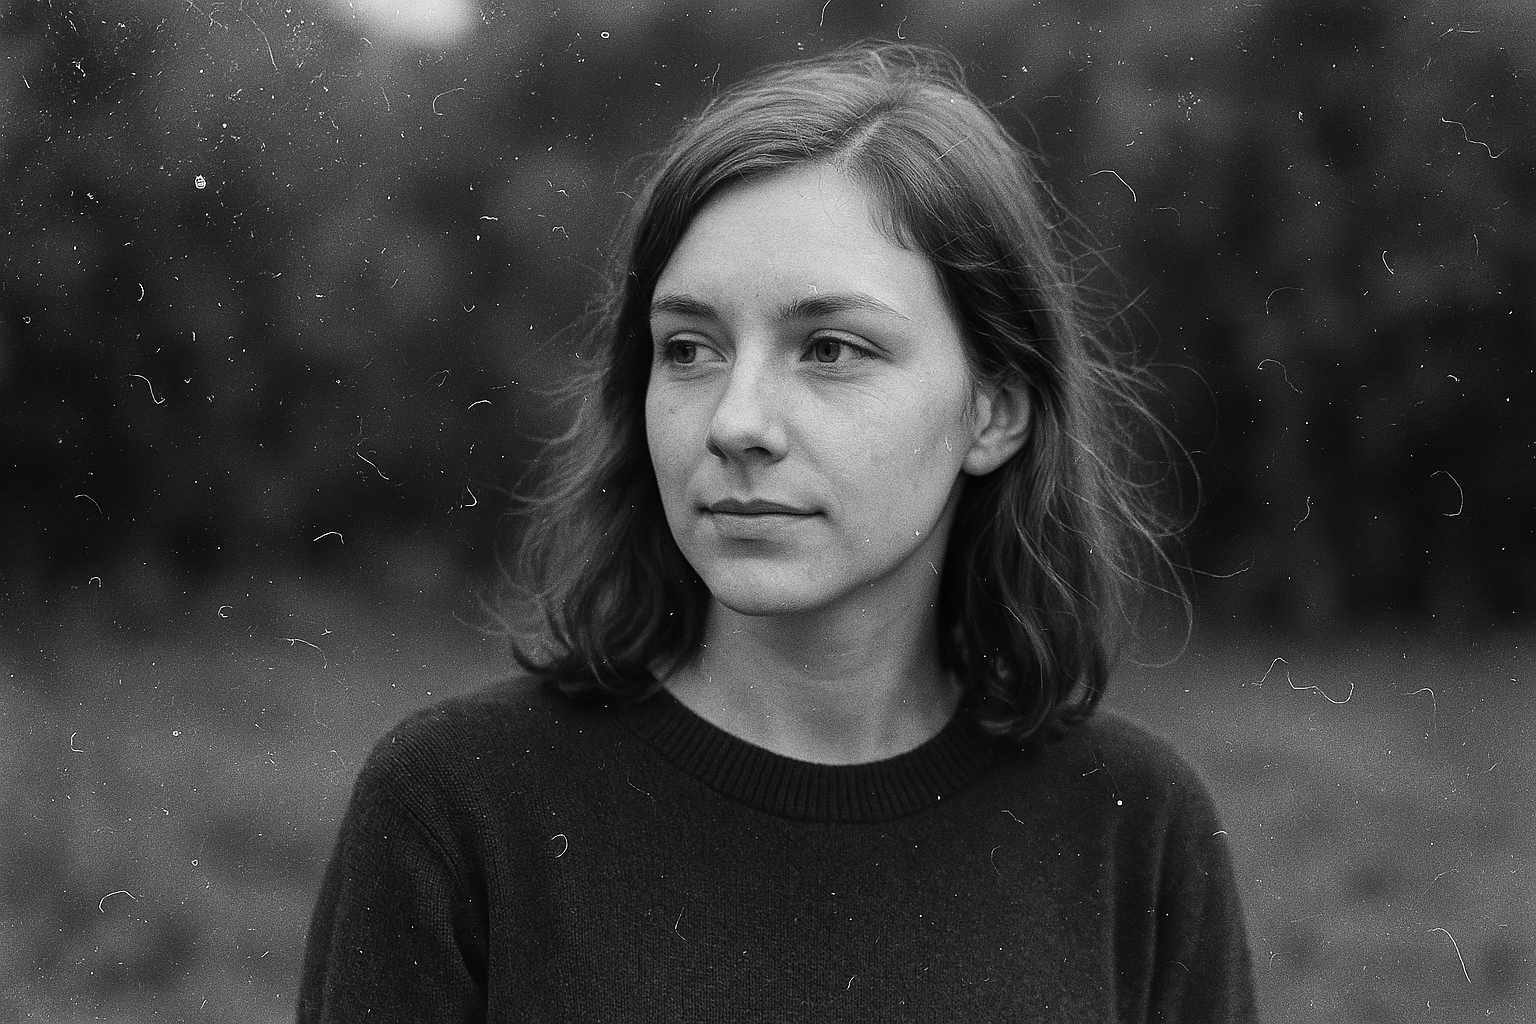
\includegraphics[width=\linewidth, keepaspectratio]{p_1.jpg}
    \caption{I prześwietlone}
\end{figure}


\subsection{Zanieczyszczenia}
Prawie że cała nasza\footnote{nie jesteśmy wszak ani naukowcami, ani lekarzami, ani ciężko chorymi. /j} codzienność
dzieje sie w niesterylnych warunkach. I jakkolwiek dla większości z nas nie jest to problem, są miejsca i sytuacje
gdy prowadzi to do pewnych problemów. W powietrzu nas otaczająym jest pełno unoszących się zanieczyszczeń: włosów, kurzu, futra etc.

Problematyczne jest natomiast osadzanie się wspomnianje powyżej materii na zdjęciach i soczewkach -- która przenosi się na
skan tworząc nieestetyczne artefakty:

\begin{figure}[H]
    \centering
    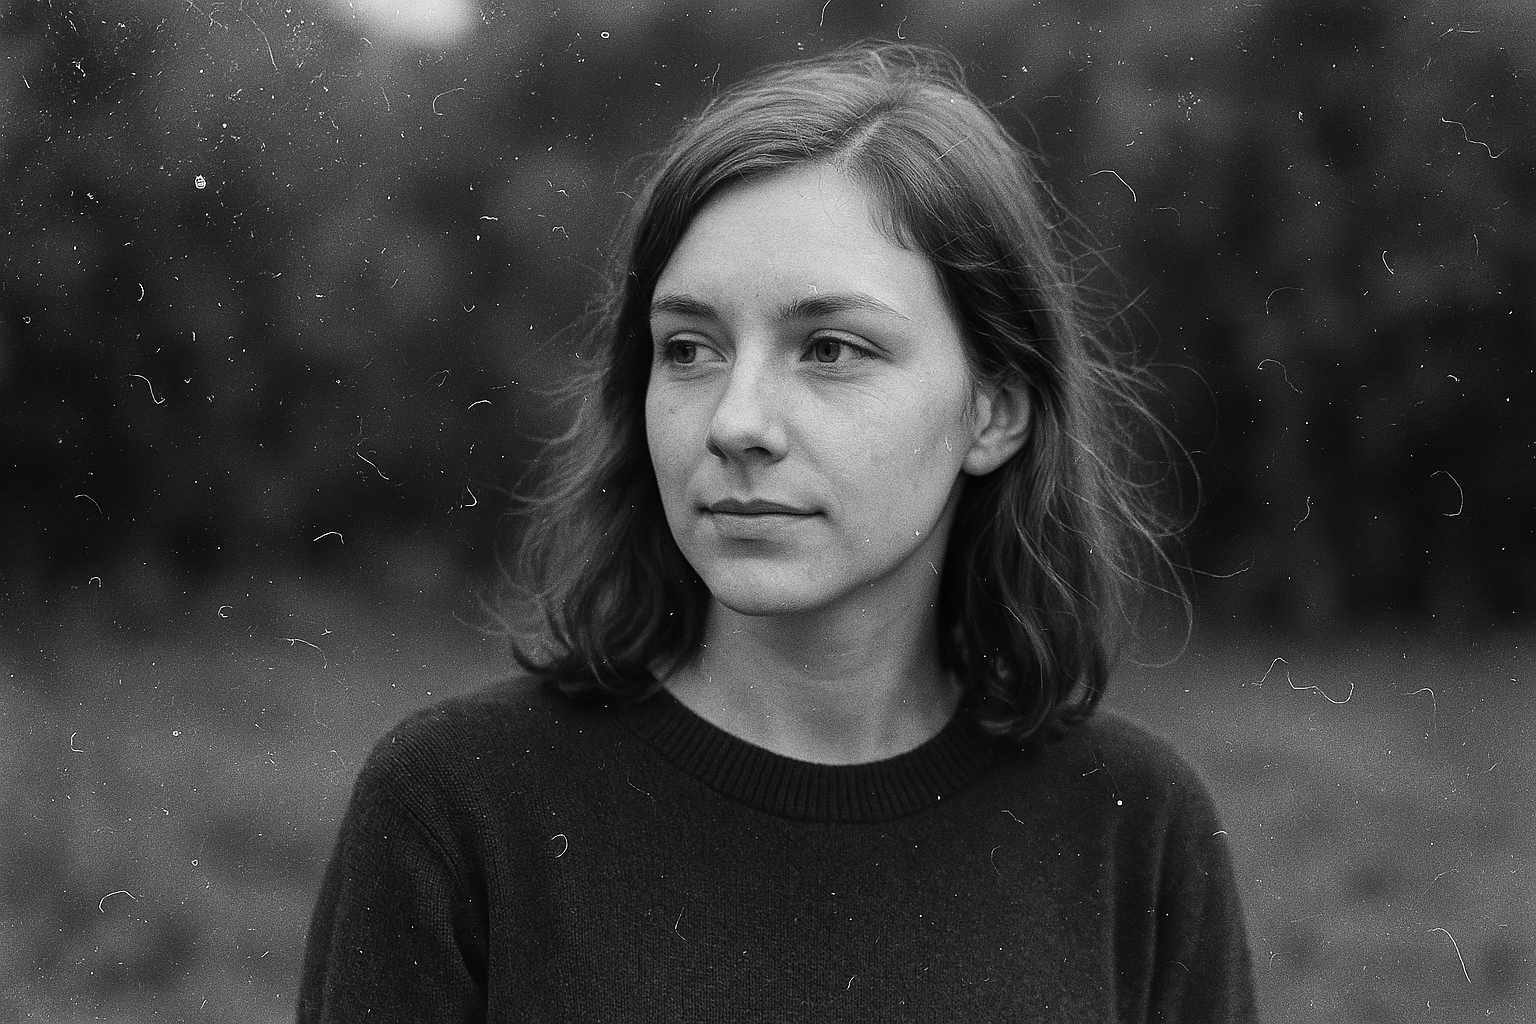
\includegraphics[width=\linewidth, keepaspectratio]{p_1.jpg}
    \caption{W skrajnych wypadkach może wyglądać to nawet tak}
\end{figure}

\begin{figure}[H]
    \centering
    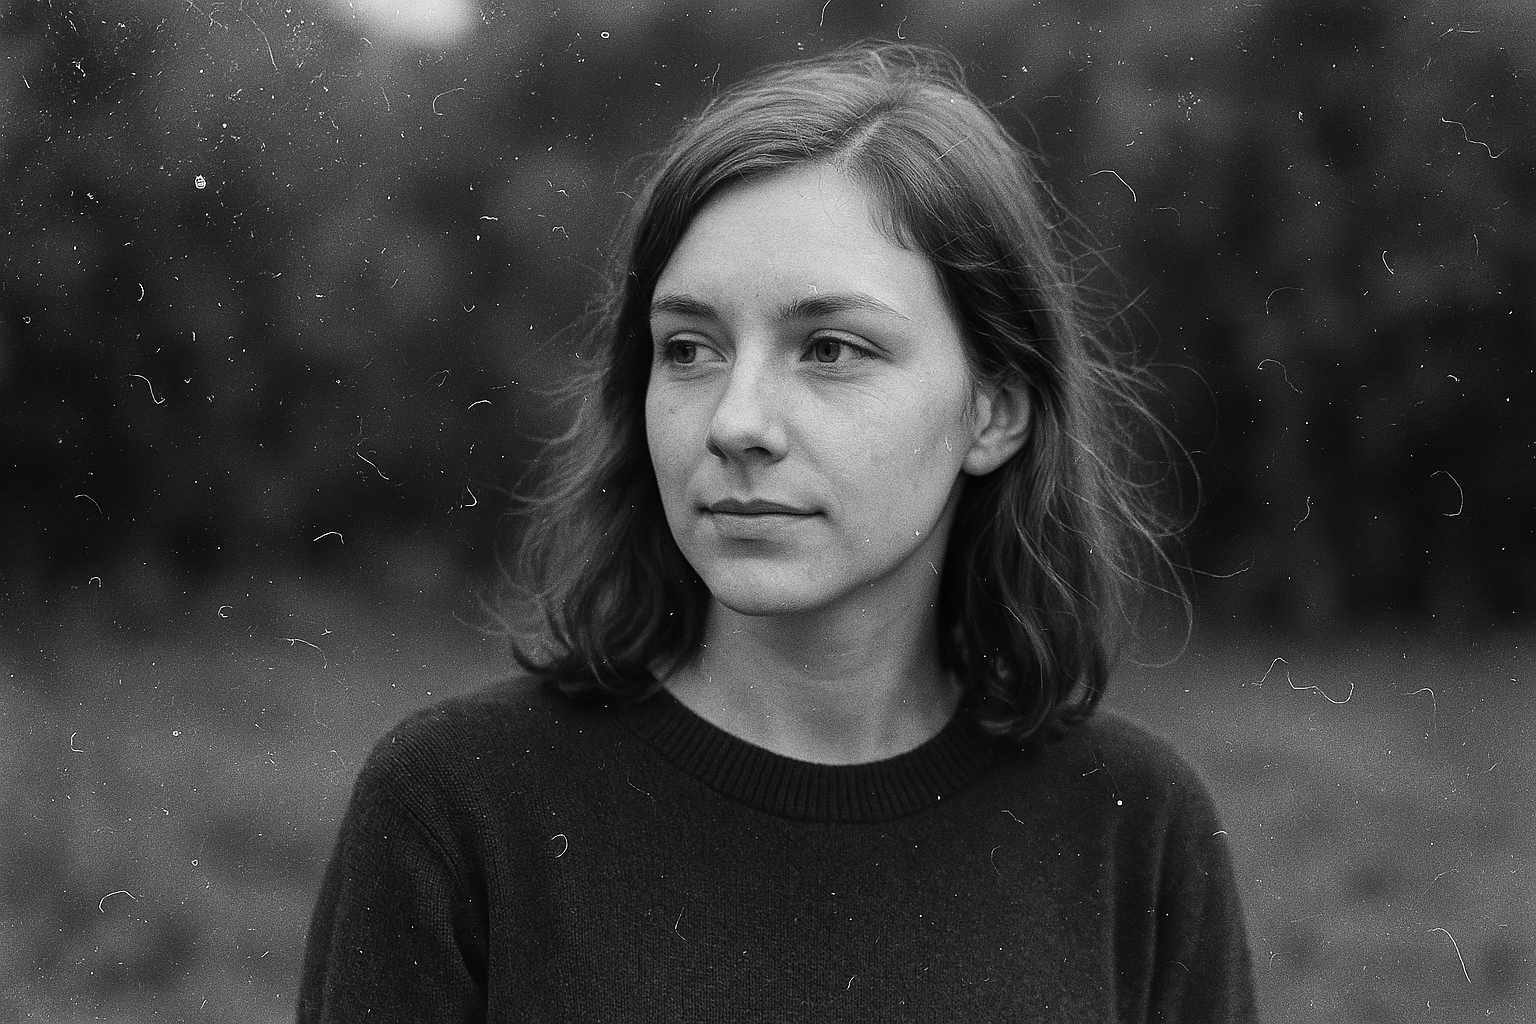
\includegraphics[width=\linewidth, keepaspectratio]{p_1.jpg}
    \caption{Choć bardziej częstym jest ten przypadek}
\end{figure}

\begin{figure}[H]
    \centering
    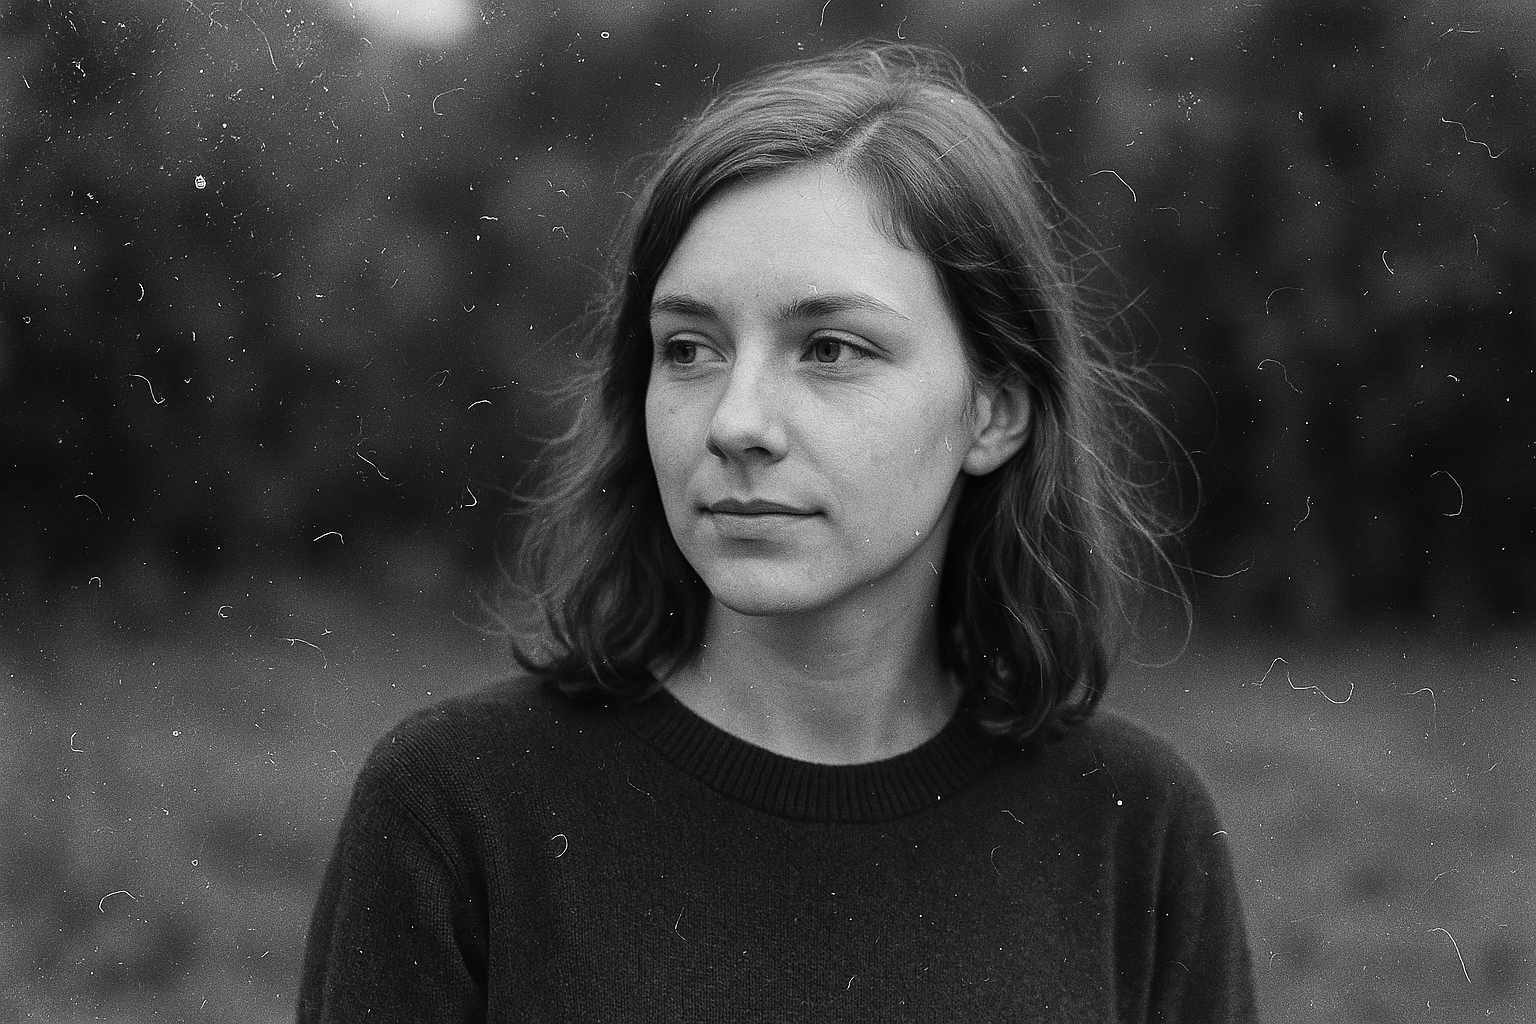
\includegraphics[width=\linewidth, keepaspectratio]{p_1.jpg}
    \caption{A także taki}
\end{figure}


\section{Program}
Zbrojni w wiedzę co chcemy osiągnąć i zapas zebranych skanów zdjęć do testów wzielismy się do pracy
nad programem.

\subsection{Yapping techniczny w subsekcjach}
bla bla bla bla bla bla






\section{Dostępność programu}
Nasz program jest programem terminalowym działającym na systemie nie starszym niż Windows 10.

Program dostępny jest dostępny na licencji \textit{bla bla} i można go znaleźć na GitHubie
pod adresem \url{https://github.com/ssk12o/PTI-Foto-Projekt}.




\newpage
\section{Wykorzystywane narzędzia}
W tej części naszego projektu korzystaliśmy z następujących narzędzi:
\begin{itemize}
    \item Programu i języka Matlab -- do analizy zdjęć;
    \item Języka c++ -- do napisania programu;
    \item Skanera minilab Noritsu HS-1800 -- do wykonywania wysokiej jakości cyfrowych skanów zdjęć wykonanych techniką analogową;
    \item Programu LibreOffice Calc -- do analizy części danych numerycznych;
    \item $\LaTeXe{}$ -- do przygotowania raportu;
    \item Google Drive -- do udostępniania plików;
    \item Github -- do udostępniania i pracy nad kodem;
    \item 7zip -- do kompresji zdjęć;
    \item Aparatów:
          \begin{itemize}
              \item Canon EOS 300 z obiektywem Tamron 28-105mm 1:4-5.6 i kliszą Fomapan 400
              \item Fujifilm FinePix L55 Digital Camera -- Black (12MP, 3x Optical Zoom)
          \end{itemize}
\end{itemize}


\section{Podział obowiązków}
Na tym etapie projektu podzieliśmy się pracą, obowiązkami i zadaniami w następujący sposób:
\begin{itemize}
    \item Bartosz Wójcik -- wykonywanie, skanowanie i analiza zdjęć; opieka merytoryczna.
    \item Katarzyna Szwed -- tworzenie, analizowanie i pisanie algorytmu; korekta raportu.
    \item Natalia Szymańska -- pisanie raportu.
    \item Patrycja Szałajko -- zarządzanie pracą zespołu, kontakt z mediami.
    \item Aleksandra Wójcik -- skanowanie zdjęć rodzinnych w celu polepszenia ich jakości w końcowych etapach projektu.
    \item Karol Sęk -- tworzenie, analizowanie i pisanie algorytmu.
    \item Michał Juszkiewicz -- tworzenie, analizowanie i pisanie algorytmu.
    \item Filip Sajko -- pisanie raportu, implementacja w \LaTeX{}.
\end{itemize}




\end{document}